\subsection*{a}
Suppose we pick 12 elements 
$\Sigma = R^{12}$ such that 
$\forall i,j \in [12]: \sigma_i \neq \sigma_j$.
Then we can construct such set 
$X$, such that $X = \Sigma$, and in this case $\forall i \in [12]: h_X(\sigma_i) = 1$.
On the other hand we can construct set X, such that 
$X intersection \Sigma = \{\}$. Moreover we can construct such X, that  any valuation of 
$(h_X(\sigma_1), .., h_X(\sigma_{12}))$ is possible, thus there could be total $2^{12}$ possible sets X, that will give a different $(h_X(\sigma_1), .., h_X(\sigma_{12}))$ valuations.\\
Suppose we pick 13 elements 
$\Sigma = R^{13}$, such that 
$\forall i,j \in [13], i \neq j, \and \sigma_i, \sigma_j \ in \Sigma: \sigma_i \neq \sigma_j$. Then  forall possible sets X 
$\exists \sigma \in \Sigma: \sigma \not \in X$. Which means valuation 
$\forall i\in [13]: h_X(\sigma_i) = 1$ is impossible, thus there is at most 
$2^{13} - 1 < 2^{13}$ possible valuations.
Suppose we pick 13 elements, where some elements are equal, such that 
$\exists i,j \in [13], i\neq j: \sigma_i = \sigma_j$. This means, that among all possible valuations 
$\{0,1\}^{13}$ i-th and j-th bits are the same, and thus total number of valuations is at most 
$\dfrac{2^{13}}{2} = 2^{12} < 2^{13}$.\\
This means, that the VC-Dim($H$)$ = 12$.

\subsection*{b}
Firstly, it is important to set up our goal. In Vapnik–Chervonenkis dimension, we should search for the largest set shattered by a hypothesis class ($H$). In this case, our $H$ is a circle and everything inside of it is valued 1. Otherwise, it is valued 0. Being so: \\
$$
h_{a,b,r}(x,y)=
        \begin{cases}
			1, & \text{if $(x-a)^2+(y-b)^2 \leq r$}\\
            0, & \text{otherwise}
		 \end{cases}
$$
\bigbreak
Proving the VC-dimension is at least 3:\\
\bigbreak
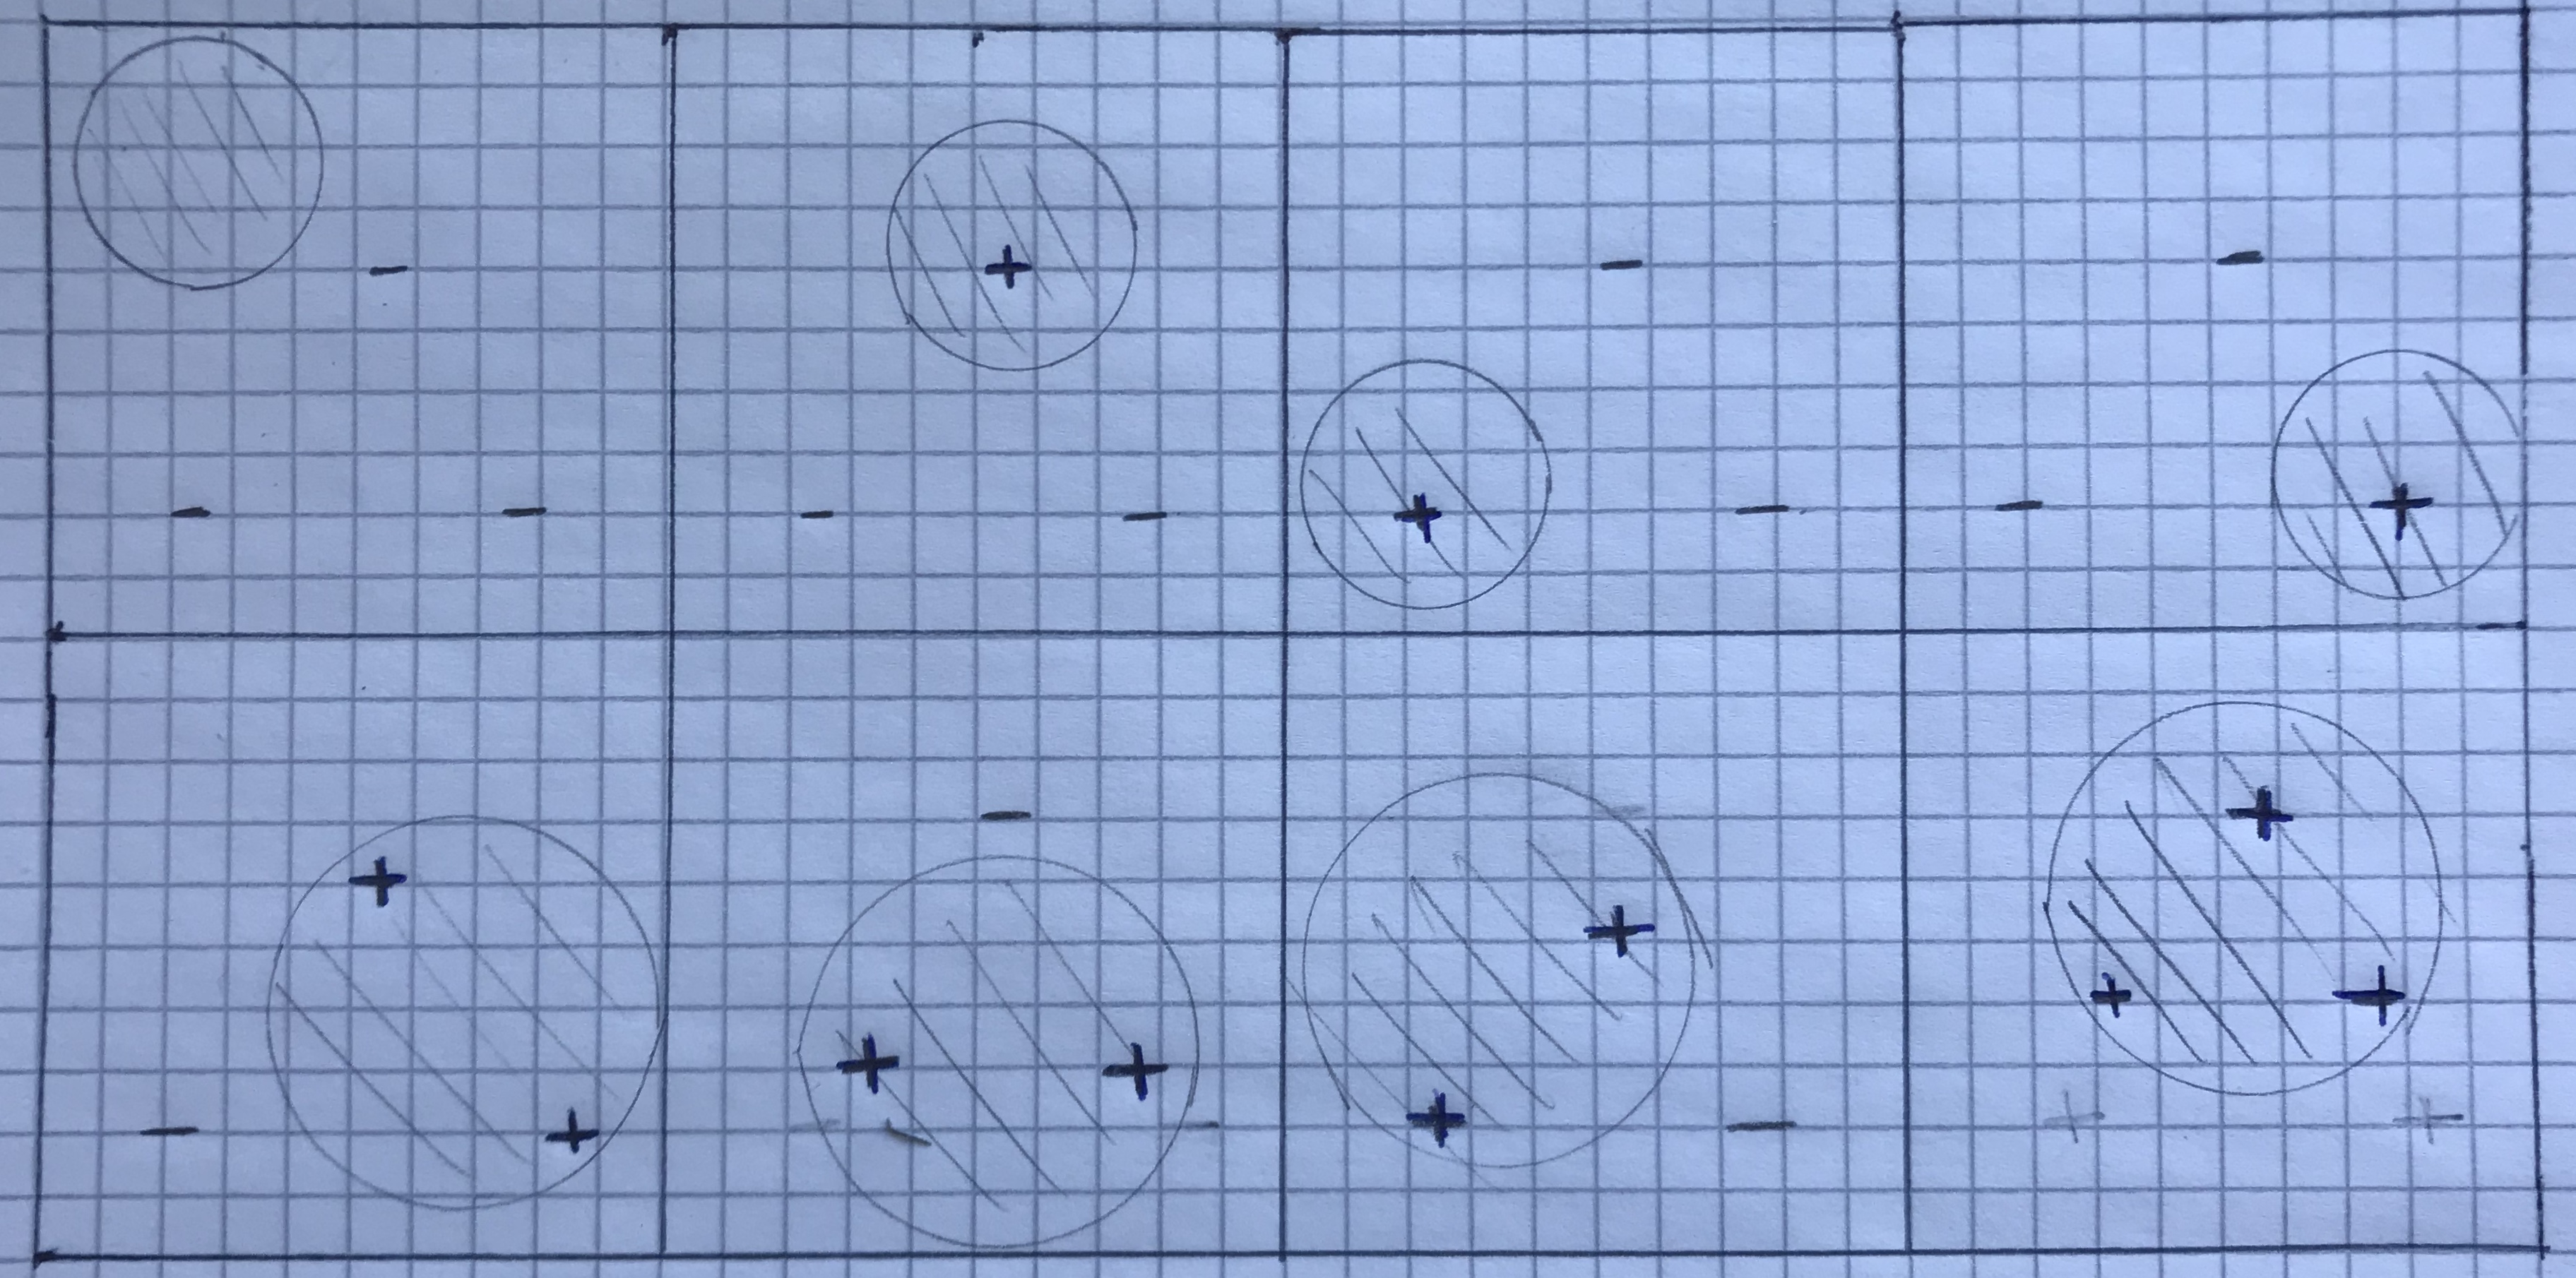
\includegraphics[width=\textwidth,height=\textheight,keepaspectratio]{3dim.jpg}\\
\bigbreak
VC-Dim is at least 3, once we can  draw a circle that have none points, that have any single point, any two points and all of them.\\
\bigbreak
Proving the VC-dimension cannot be 4:\\
\bigbreak
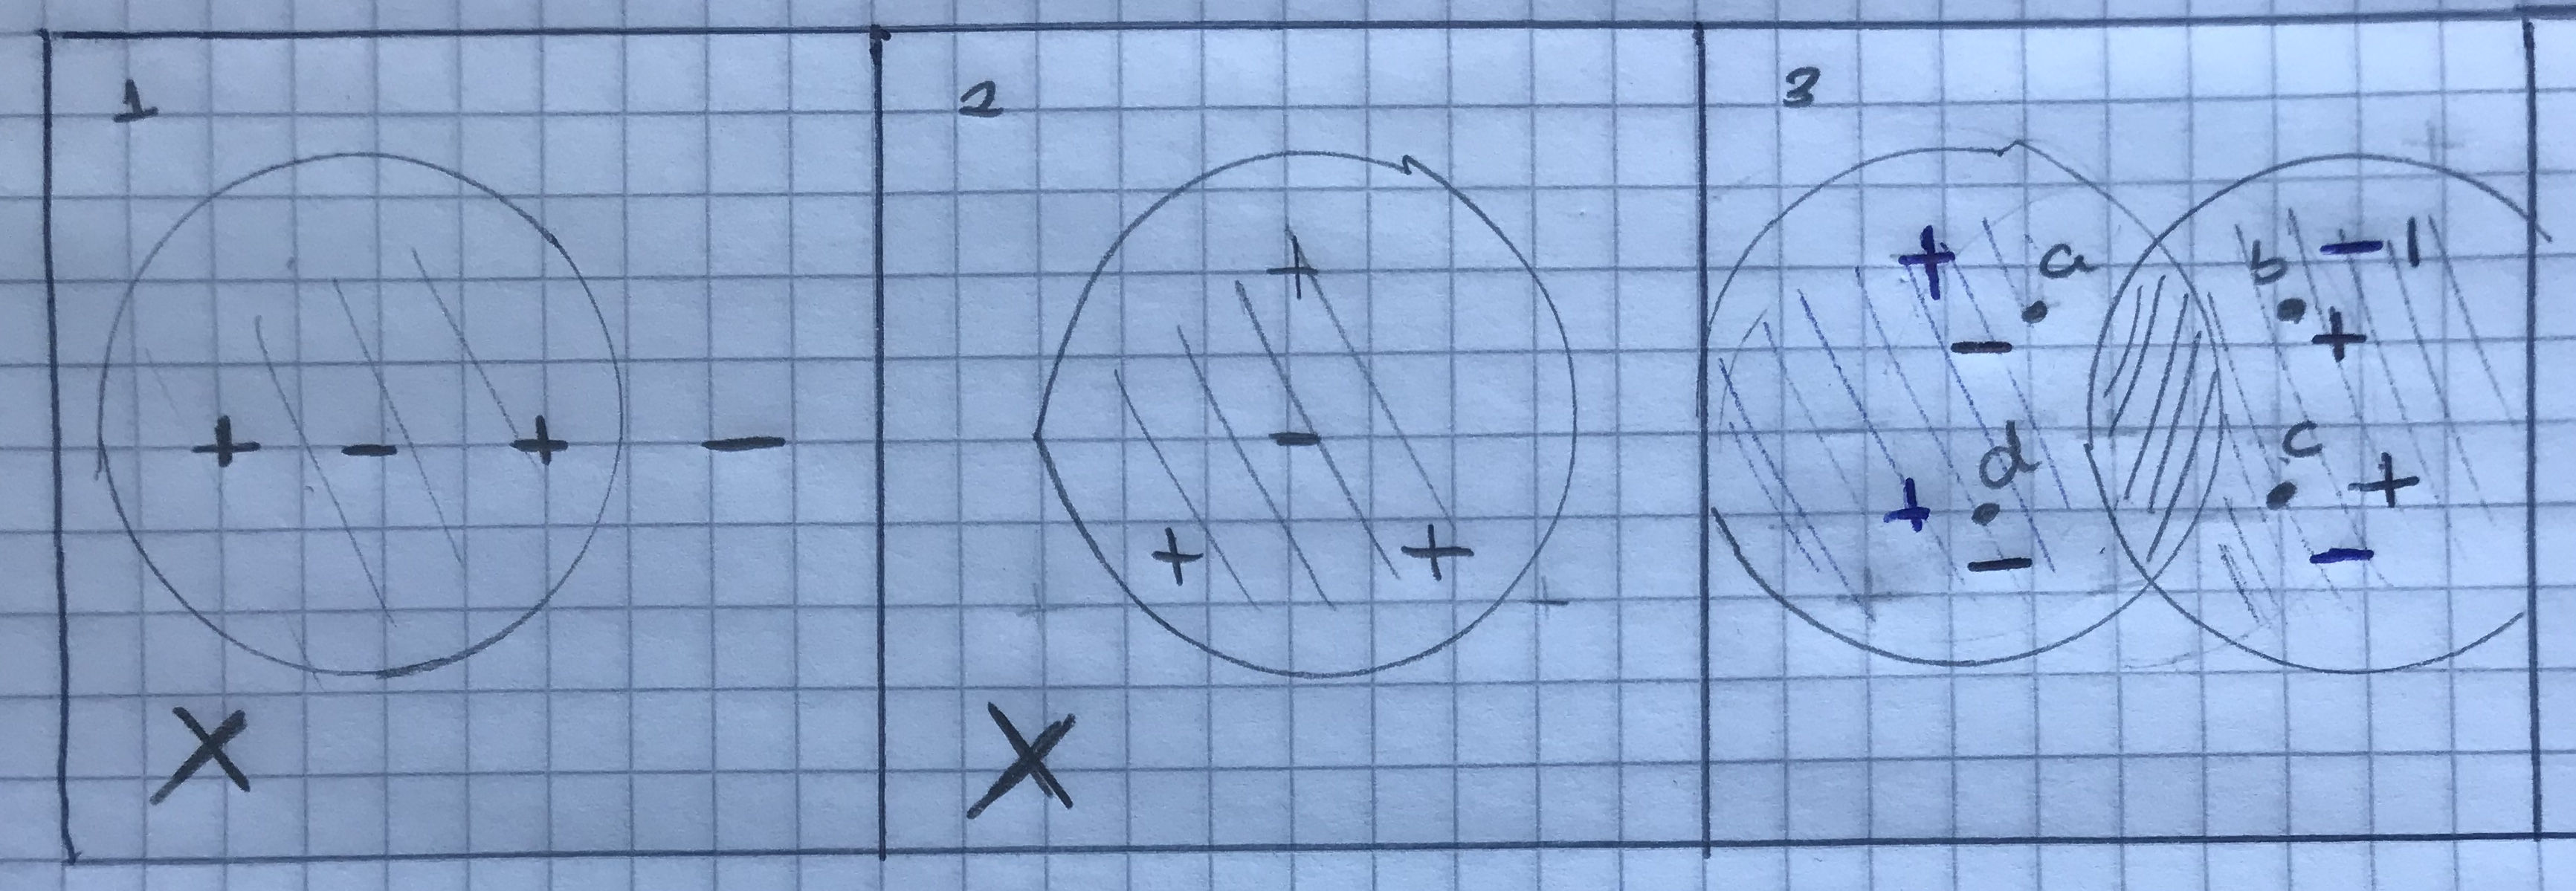
\includegraphics[width=\textwidth,height=\textheight,keepaspectratio]{4dim.jpg}
\bigbreak
VC-Dim cannot be four for the following three reasons:
\begin{enumerate}
  \item Labeling, for instance, $+ - + -$ in this colinear points example is impossible. Several others example with similar arrangement fit in the same explanation. 
  \item Being the convex hull of the four points a triangle, is impossible for the outside points be + and the inside point be -.
  \item Lastly, being the convex hull a quadrilateral defined by points {$a,b,c,d$}, it is not possible to exist a circle that involves $a,c$ and another circle that involves $b,d$. If so, the symmetric difference would consist of 4 disjoint regions, which is indeed impossible for circles.
\end{enumerate}
\bigbreak
Therefore, we can conclude that VC-Dim($H$)$ = 3$. 
